 \documentclass[conference]{IEEEtran}
\IEEEoverridecommandlockouts
% The preceding line is only needed to identify funding in the first footnote. If that is unneeded, please comment it out.
\usepackage{cite}
\usepackage{amsmath,amssymb,amsfonts}
\usepackage{algorithmic}
\usepackage{graphicx}
\usepackage{textcomp}
\usepackage{xcolor}
\usepackage{graphbox}
\usepackage{tabularx}
\usepackage{amsmath}
\usepackage{amssymb}
\usepackage{amsfonts}
\usepackage{svg}
\DeclareMathOperator*{\argminB}{argmin} 
\DeclareMathOperator*{\argmaxB}{argmax} 
\newcommand\norm[1]{\left\lVert#1\right\rVert} 
\def\BibTeX{{\rm B\kern-.05em{\sc i\kern-.025em b}\kern-.08em
    T\kern-.1667em\lower.7ex\hbox{E}\kern-.125emX}}
\begin{document}

\title{Detecting Fashion Apparels and their Landmarks\\
\thanks{Thanks to Dataperformers for providing the resources to accomplish this project.}
}



\author{\IEEEauthorblockN{1\textsuperscript{st} Himani Saini}
\IEEEauthorblockA{\textit{Department of Computer Science and}\\
{\textit{Software Engineering}} \\
\textit{Concordia University}\\
Montreal, Canada \\
himmi.saini@gmail.com
}
\and
\IEEEauthorblockN{2\textsuperscript{nd} Viral Thakar}
\IEEEauthorblockA{\textit{Department of Electrical and} \\
\textit{Computer engineering} \\
\textit{Concordia University}\\
Montreal, Canada \\
v\_thakar@encs.concordia.ca
}
\and
\IEEEauthorblockN{3\textsuperscript{rd} Riddhi Dasani}
\IEEEauthorblockA{\textit{Dataperformers} \\
Montreal, Canada \\
riddhi@dataperformers.com
}
\and
\IEEEauthorblockN{4\textsuperscript{th} Jia Yuan Yu}
\IEEEauthorblockA{\textit{Concordia Institute of Information System Engineering} \\
\textit{Concordia University}\\
Montreal, Canada \\
jiayuan.yu@concordia.ca
}
}

\maketitle

\begin{abstract}
Apparel landmarks are the functional key-points on the apparels that can be used for a more discriminative visual analysis of the apparel images. 
Such a framework can facilitate apparel alignment in displaying apparel images on the websites for recommendation systems, apparel image retrieval, apparel style transfer, trend analysis or help build a system to ensure dress code in a particular environment. However, challenges such as background clutter, human poses, scales apparel variation and lighting can render such a task difficult. We present a conceptually simple, flexible, and general framework for apparels' landmark detection that can also be simultaneously used for apparel detection. In addition to the position of the landmarks in the apparels, we also classify the landmarks as visible or occluded in the same framework. We perform all these tasks in parallel using multi-task learning. Our proposed convolutional neural network is end-to-end differentiable and simple to train, since all these tasks are performed on the same architecture without any additional parameters to learn. The fashion landmark detection task is similar to joint localization and detection problems like human pose estimation, hence our approach extends stacked hourglass architecture, originally proposed to solve human pose estimation. 
Over the past few years, many modifications have been proposed to improve this architecture. We also compare the performances of some of these different variations of stacked hourglass architectures. These architectures leverage both global and local features captured by the deep convolutional neural networks to better localize the apparel in the image as well as the landmarks in those apparels.
\end{abstract}

\begin{IEEEkeywords}
E-commerce, Fashion Analysis, Computer Vision, Convolutional Neural Network
\end{IEEEkeywords}

\section{Introduction}
In the past few years, visual analysis of fashion items have received a lot of interest from the research community because of the gamut of applications ranging from apparel classification \cite{huang2015cross, he2016identity, liu2016deepfashion}, retrieval \cite{liu2016fashion, fu2012efficient}, recommendation \cite{packer2018visually, agarwal2018personalizing}, attribute prediction \cite{liu2016deepfashion, wang2018attentive}, style discovery and extraction \cite{simo2016fashion, gabale2018extract}, outfit generation \cite{nakamura2018outfit}, to name a few. Hence research in this field brings a lot of value to the fashion e-commerce industry, which is estimated to be \$ 712.9 billion by 2022 \cite{FashionTrends}. The advent of deep convolutional neural networks and the availability of powerful computational resources have enabled researchers to draw meaningful information from the fashion images. 
% This research is further advanced by the availability of the large-scale fashion datasets like Fashion MNIST \cite{FashionMNIST}, DeepFashion \cite{liu2016deepfashion}, FashionAI \cite{FashionAI}, DeepFashion2 \cite{DeepFashion2}, PaperDoll \cite{PaperDoll}, etc. to tackle different tasks.  
Fashion landmark detection is another such task that can bring enormous value to this domain. These fashion landmarks are the key-points located at the functional regions of the apparels e.g., neckline, cuff, etc. and much like human key-points in the problem of human pose estimation \cite{andriluka14cvpr}, they can represent the configuration of an apparel by itself or on a human body (Fig 1). These functional regions can better distinguish design, pattern or texture and category of the apparels. They can facilitate tasks like  tracking, localized auto-editing of apparel images, or providing better insights into fashion trends, style analysis, etc. in order to build more customized recommendation systems. One of the key applications of such landmarks is to create a consistently-aligned inventory to boost the appeal of the apparel images on the websites. Detecting landmarks can help making sure that all the apparels displayed on the website are uniform in size and their corners, contours and angles are carefully aligned with respect to each other as well as to the alignment guidelines of the website. 
Another key application of these landmarks is to develop a  system to ensure the dress codes as per the occasion and environment. The relationship of these detected landmarks among each other can give meaningful insights on the type of apparel a person is wearing which can be checked against the established dress-code to flag the anomalies. Hence detecting landmarks can bring effectiveness in both social and commercial fashion domains.

However, localization of these landmarks is a challenging problem because of the diversity of apparels, background clutter, occlusion, scale variation, frequent style changes, etc. In addition to these variations, the images also differ in their environment e.g., the images from an e-commerce platform are aesthetically and technically superior \cite{talebi2018nima} to the images collected from a social media platform. Moreover, these images also exhibit human body and pose variation since people across different platforms take pictures in different poses and photos are
taken from different camera viewpoints and focal lengths. On one hand, local details on apparel images like collar and cuff are more important to localize these landmarks, while on the other hand, global attributes of the apparel itself are more important in order to solve the spatial relationships among those landmarks, i.e., the left and right collar or the left and right sleeve.
\begin{figure}[ht]
%     \begin{adjustbox}{width=\textwidth,center}
    % \begin{adjustbox}{center}
    \centering
        \begin{tabular}{ccc}
            {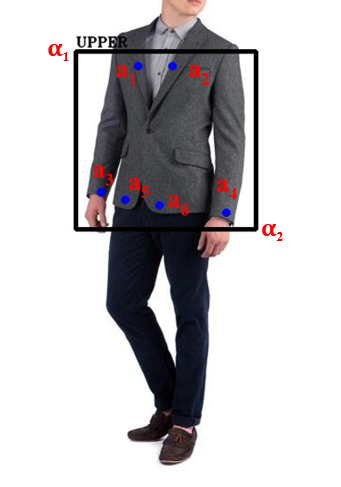
\includegraphics [width = 0.9in, height= 3cm]{images/anno_upper.PNG}} & 
            {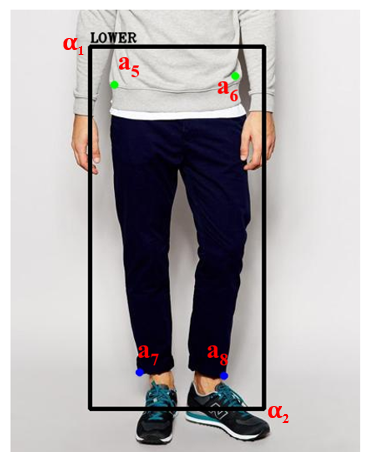
\includegraphics [width = 0.9in, height= 3cm]{images/anno_lower.PNG}} & 
            {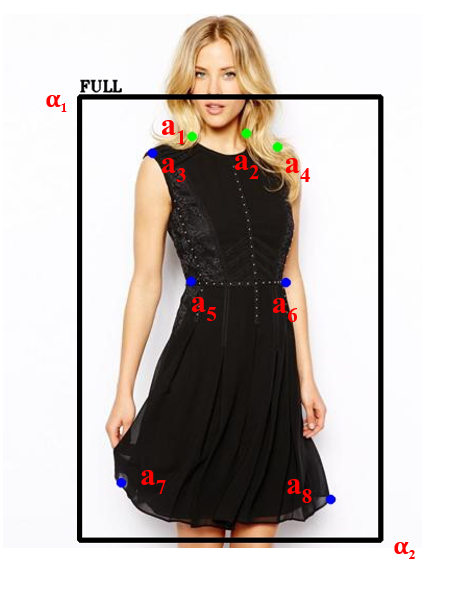
\includegraphics [width = 0.9in, height= 3cm]{images/anno_full.PNG}} \\
        \end{tabular}
        \caption{Images for upper-body apparel, lower-body apparel and full-body apparel with annotated attributes as well as the bounding boxes. Blue dots  represent the visible landmarks and the green dots represent the occluded landmarks on the apparels.}
\end{figure}
In this work, we solve this problem using stacked hourglass  architecture \cite{newell2016stacked}, which is a dominant approach forming the back-bone of many leading approaches for MPII dataset \cite{andriluka20142d}, a benchmark for human pose estimation. The key aspect of the stacked hourglass architecture is that it extracts and consolidates the features across all scales, leveraging both local and global information present in the images to learn the spatial relationships among the different locations of the image. It does so using repeated bottom-up and top-down processing, that constitutes its hourglass shape. Furthermore, this architecture is extended by stacking multiple hourglasses next to each other, which enables cascaded inferences along with intermediate supervision. Over years, many modifications have been made to this architecture. Two such variations are pyramid residual networks \cite{yang2017learning} and cascaded pyramid fusion \cite{zhang2019human}. These architectures were built to employ specific properties of convolutional neural networks like multi-scale features maps, etc. in order to further improve the predictions.
In addition to the landmarks, we also localize the top-left and bottom-right corners of the bounding boxes for each category of the apparel, without any need of anchor boxes in order to provide an enriched fashion analysis (Fig 1). We train this network using multi-task losses for each of these tasks. Our approach is motivated by Mask R-CNN in that sense, but unlike Mask R-CNN, which introduces branches to the base network and adds more parameters specific to learning specific tasks, our approach uses the same features to perform all these tasks in parallel.
The contributions of this work are as follow:
\begin{itemize}
    \item We present a unified framework for apparel landmark detection, that can simultaneously be used for apparel detection.
    \item We test our proposed approach on the state-of-the-art fashion landmark datasets, i.e., DeepFashion \cite{liu2016deepfashion}.  
    \item We also compare the performance of two different variations of the stacked hourglass architecture for landmark detection. 
\end{itemize}

\section{Related Work}

Initial work on fashion landmark detection \cite{liu2016fashion} takes bounding boxes of the apparel images at the training as well as testing time. In addition to input images, it takes 8 labels, i.e. upper, lower or full-body apparel categories, normal, medium or large poses and medium zoom-in or large zoom-in variations to learn pseudo-labels representing the relationship of one sample image to another. These pseudo-labels are then used to learn and refine the landmark localization in a cascaded network and learn the apparel configuration.

 The next work \cite{yan2017unconstrained}, takes full images as an input as well as zoom-in or zoom-out labels to inject high-level human knowledge into the network. It uses \textit{Selective Dilated Convolution} to handle scale discrepancies and \textit{Hierarchical-Recurrent Spatial Transformer} network, as an attention mechanism to ignore the background clutter. Selective dilated convolution use dilated filters instead of the traditional convolutional neural network filters in order to increase the receptive field of the image, keeping the same number of parameters. This helped in evaluating images at different scales, using 4 different dilation values. Hierarchical-recurrent spatial transformer networks on the other hand are the modification of spatial transformer networks \cite{jaderberg2015spatial}, which are used to encode a mechanism to handle affine distortions in the image. It learns the geometric transforms on the input image to focus more on the object in the image, ignoring the background. But since fashion images provide a lot of variations in terms of poses and background clutter, a series of geometric transformations are progressively learnt for all the landmarks in an hierarchical manner. In addition to that, so as to not learn the same transforms again, a recurrent state of the transforms is saved for each landmark. \cite{liu2016fashion, yan2017unconstrained} employ direct regression over the fully connected layers, which is a highly non-linear problem and lacks the generalization ability \cite{lin2013network}. When the features obtained after convolutional layers are flattened, there is a huge loss in the spatial features of those feature maps. Instead, recent approaches for both human pose estimation \cite{yang2017learning, chen2017adversarial, chu2017multi} and fashion landmark detection \cite{wang2018attentive} predict heat-maps or confidence maps of positional distribution of each landmark, given the input image.

  The recent approach \cite{wang2018attentive} encodes the knowledge over fashion apparels by developing a domain specific grammar to learn kinematic and symmetric relations between apparel landmarks. \textit{Bidirectional Convolutional Recurrent Neural Network} is used for message passing over the learned grammar. It also uses two attention mechanisms: one that is landmark-aware and involving domain-knowledge, and another directly focusing on the category relevant image regions.  While all these approaches work with different efficiencies, they produce features specific to fashion landmarks only and cannot be used for other tasks.

 During our research, we realized that fashion landmark detection is similar to human pose estimation in terms of the objective, yet is more challenging because of many reasons. The human key-points in the images are subject to rigid deformations, whereas the landmarks in fashion items are subject to non-rigid deformations like stretching and shrinking. Furthermore, apparels have a much larger scale variation than human poses. A same category of apparel can have it's landmarks at different places on human body. e.g., A dress can be a full-body dress, a medium-length dress or a short-length dress, making the localization of the dresses' landmarks more difficult. Also, local regions of fashion landmarks have larger appearance variations than those of human key-points. e.g., An upper-body woman apparel can be a T-shirt, a camisole, a racer back top or a tank top. Another challenge comes from the uneven number of landmarks in different apparels. In human pose estimation, the number of key-points are fixed throughout the dataset, (fifteen in MPII \cite{andriluka14cvpr}). Whereas, in fashion landmarks detection, different apparels have different number of landmarks. e.g., In DeepFashion \cite{liu2016deepfashion}, an upper-body apparel has six landmarks, a lower-body apparel has four landmarks and a full-body apparel has eight landmarks. Even if both upper and lower-body apparels are present in an image, the annotations are provided only for one of these categories. This makes it difficult for the network to learn the landmarks to predict in an image.
 In human pose estimation, the global cues captured by the later stages of convolutional neural network provide the spatial context for the localization of the key-points with respect to each other. Hence, the key-points that are difficult to localize and differentiate, e.g., shoulders and elbows, are learned with respect to the key-points that can be localized with greater confidence e.g., head or neck. But in case of fashion landmarks, the position of the sleeve can be anywhere on the arm with respect to the collars. So, properly learning the contextual information is more important for localization of fashion landmarks.

\section{Methodology}

\subsection{Problem Formulation}
Let $X$ be the set of images, where $i^{th}$ image $x^i \in X$ contains one fashion item to be annotated with the fashion attributes. Let $\textsc{Z}$  be the set of all the pixel locations $(u,v)$ in the coordinate space $\mathbb{R}^{m \times n \times C}$ of $x^i$, where $(m \times n)$ and $C$ are the resolution and number of channels of $x^i$ respectively and $u \in \{1, \ldots, m\}$ and $v \in \{1, \ldots, n\}$. Let $Y$ be the label set representing the corresponding fashion attributes $y^i \in Y$. $y^i$ consists of a vector of all fashion attributes, namely, a class label $\beta \in \{1, \dots, \tau\}$ describing the type of the apparel using $\tau$ class labels; two opposite corner locations $\alpha_1, \alpha_2 \in Z$ (top-left and the bottom-right) localizing the apparel item in the image; and an ordered set of $P$ fashion landmarks $(a^i_1, \dots ,a^i_P)$, such that, $y^i = (\beta^i, \alpha^i_1, \alpha^i_2, a^i_1, \dots ,a^i_P)$. In DeepFashion \cite{liu2016deepfashion}, $\beta \in \{1,2,3\}$ where the values 1, 2 and 3 represent the upper-body apparels (T-shirt, top, etc.), lower-body apparels (pants, shorts, etc.) and full-body apparels (dresses, jumpsuits, etc.) respectively. It has $P=8$ landmarks, which are ordered as left collar, right collar, left sleeve, right sleeve, left waist, right waist, left hem, right hem. Each fashion landmark $a^i_p$  is a three dimensional vector $a^i_p = (u,v,\gamma)$, where $(u,v) \in Z$ indicates the location of the landmark and $\gamma \in \{0,1\}$ represents the visibility flag such that the values 1 and 0 indicate the visible and the occluded landmarks respectively. 

% ($p^{th}$ fashion landmark for $x^i$)

Let $S_N = \{(x^1, y^1), \dots, (x^N, y^N)\}$ be the training set containing $N$ apparel images, where $(x^i,y^i) \in (X, Y)$. The objective is to learn a function $\varphi_{S_N}$, that predicts the fashion attributes $\hat{y^i}$ for given $x^i$. This function $\varphi_{S_N}$ consists of a stacked hourglass convolutional neural network, followed by a post processing function  specific to different components of $\hat{y}^i$.

For $x^i$, a sequence of ground-truth heat-maps is generated by assigning a discreet 2D gaussian  to $(u, v)$ and its neighbouring locations up to certain width. This produces a surface whose contours are concentric circles with the pixel at landmark location receiving the highest gaussian value, creating a soft peak, decreasing symmetrically as the distance from that location increases. Using a convolutional neural network, a sequence of output heat-maps $\hat{\mathbb{H}}^i= \{\hat{h}^i_1,\dots ,\hat{h}^i_P \}$ is computed for $x^i$, which are refined via heat-map regression using the mean squared loss  between the set of output heat-maps and ground-truth heat-maps for all the images in $S_N$ as: 
% 
\begin{equation}
\mathcal{L}^{N}_P \big( \mathbb{H} , \hat{\mathbb{H}}\big) = \frac{1}{N}\frac{1}{P} \sum_{i = 1}^{N} \sum_{p = 1}^{P} \norm{ h^i_{p} - \hat{h}^i_p }^2,
\end{equation}
% 
where $\norm{h^i_{p} - \hat{h}^i_{p}}^2$ is the $l_2$ loss between the ground and the predicted $p^{th}$ heat-map for $x^i$. The estimated landmark locations are determined by computing the location of the first brightest pixel, i.e. the pixel with the maximum value in the corresponding heat-map. 

Also, for $x^i$, a sequence of ground-truth visibility-maps $\mathbb{G}^i= \{ g^i_1,\dots ,g^i_P \}$ is generated for $P$ landmarks to encode each landmark's visibility information as a set of $P$ binary maps. In each $g^i_p$, if the visibility flag $\gamma$ in $a^i_p$ is 1, the values within a certain width around the ground truth location $(u , v)$ are set to 1 and the values for the remaining background are set to 0. This is to ensure that each of the approximate position in the corresponding heat-map of the landmark has the same visibility state.  Hence for the occluded landmarks $g^i_p$ remains a zero-matrix. A sequence of output visibility-maps $\hat{\mathbb{G}}^i= \{\hat{g}^i_1,\dots ,\hat{g}^i_P \}$ are computed for $x^i$ and refined using the pixel-wise binary cross entropy loss (BCE) between the predicted and output visibility-map as:
% 
\begin{equation}
  \Lambda ( g^i_{p} , \hat{g}^i_p) = - \sum_{q = 1}^{m'} \sum_{r = 1}^{n'}{(\lambda^i_{p_{q,r}} \log(1 - \hat{\lambda}^i_{p_{q,r}})) }.
%   + (1 - \lambda^i_{p_{q,r}})\log(1 - \hat{\lambda}^i_{p_{q,r}}))},
\end{equation}
%
where $\lambda^i_{p_{q,r}}$ and $\hat{\lambda}^i_{p_{q,r}}$ respectively represent the probability of landmark's presence at the location $(q,r)$  of the ground-truth visibility map $g^i_p$ and predicted visibility map $\hat{g}^i_p$. Hence BCE loss over $S_N$ is given as, such that,  
% 
\begin{equation}
  \mathcal{V}^N_P (\mathbb{G}, \hat{\mathbb{G}}) = - \frac{1}{N} \frac{1}{P} \sum_{i = 1}^{N} \sum_{p = 1}^{P} \Lambda (g^i_{p} , \hat{g}^i_p),
\end{equation}
%
The final predictions of the visibility flag of the landmarks is determined by computing the first maximum pixel's value and then classifying the visibility flag as visible or occluded based on 0.5 threshold.
% % 
% \begin{align}
% \hat{\gamma}^i_p &= 
%     \begin{cases}
%       0, & \text{if} \;\; \max{(\hat{g}^i_p)} < 0.5 \\
%       1, & \text{otherwise}
%     \end{cases} ,\; \; p \in (1, \dots, P).
% \end{align} 
% % 
% This $\hat{\gamma}^i_p$ value obtained from $\hat{g}^i_p$ is the estimated visibility of the $p^{th}$ landmark in $(\hat{a}^i_1, \dots ,\hat{a}^i_P)$ for $x^i$. Hence the output landmarks are $(\hat{a}^i_1,\dots \hat{a}^i_P)$, where $\hat{a}^i_p = (\hat{u}^i_p, \hat{v}^i_p,\hat{\gamma}^i_p)$.

Similar to the heat-maps, locations of the top-left and the bottom right corners $\alpha^i_1,\alpha^i_2$ localizing the apparel in the image $x^i$ are estimated via heat-map regression. For $x^i$, a sequence of ground-truth heat-maps $\mathbb{O}^i= \{ o^i_1, o^i_2 \}$ is generated for $\alpha^i_1, \alpha^i_2$ and the output heat-maps $\hat{\mathbb{O}^i}= \{ \hat{o}^i_1, \hat{o}^i_2 \}$ are computed and refined using $l_2$ loss as :
% 
\begin{equation}
\mathcal{B}^{N}_2 \big( \mathbb{O} , \hat{\mathbb{O}}\big) = \frac{1}{N}\frac{1}{2} \sum_{i = 1}^{N} \sum_{j = 1}^{2} \norm{ o^i_{j} - \hat{o}^i_j }^2,
\end{equation}
% 
The output locations of the corners  $\hat{\alpha^i_1}, \hat{\alpha^i_2}$ are also determined by computing the location of the first brightest pixel.
% \hat{\alpha}^i_j &= \bigg( \max(\hat{o}^i_j) \bigg)_{q,r} ,\; \; j = 1,2, \; \; (q,r) \in Z.
% \end{align} 
% 
% % 
% \begin{equation}
% \begin{split}
% \hat{\alpha}^i_j &= \argmaxB \; (\hat{o}^i_j),\; \; j = 1,2 
% \end{split}
% \end{equation}
% % 
%

Corresponding to the each of the bounding box locations $\alpha^i_1,\alpha^i_2$ of image $x^i$, a sequence of binary class-map $\mathbb{T}^i= \{t^i_{11},t^i_{12}, t^i_{21},t^i_{22}, \dots, t^i_{\tau1} , t^i_{\tau2}\}$ of each class is created indicating the class that corner location belongs to. These class-maps are created in the similar manner as of the visibility maps, i.e., in each class-map, values within a certain width around the mapped ground truth location are set to 1 and the values for the remaining background are set to 0. Hence the class-maps to which the corner points do not belong are the zero-matrices. These class-maps are created to ensure that each of the approximate corner location in the corresponding heat-map of the corner belongs to the same class.
The sequence of output class-maps $\hat{\mathbb{T}^i}= \{\hat{t}^i_{11},\hat{t}^i_{12}, \hat{t}^i_{21},\hat{t}^i_{22}, \dots, \hat{t}^i_{\tau1} , \hat{t}^i_{\tau2}\}$ are computed and are refined using BCE loss as:
% 
\begin{equation}
  \mathcal{C}^N_{\tau} (\mathbb{T}, \hat{\mathbb{T}}) = - \frac{1}{N} \frac{1}{\tau \times 2} \sum_{i = 1}^{N} \sum_{j = 1}^{{\tau}} \sum_{j' = 1}^{2} \Lambda(\;t^i_{jj'} \; , \; \hat{t}^i_{jj'}\;),
\end{equation}
The prediction of the class of each corner $\alpha^i_1$ and $\alpha^i_2$ localizing the apparel in the image is determined by getting the maximum pixel's value and then assigning the binary classification flag. The class is assigned to the apparel if both the corners belong to the same class. 
The total loss is given by $L^N$, as:
%
\begin{equation}
\begin{split}
   L^N = \nu_1 \; \mathcal{L}^{N}_P \big( \mathbb{H} , \hat{\mathbb{H}}\big) + \nu_2 \; \mathcal{V}^N_P (\mathbb{G}, \hat{\mathbb{G}}) + \nu_3 \;\mathcal{B}^{N}_2 \big( \mathbb{O} , \hat{\mathbb{O}}\big) 
\\
+ \nu_4 \; \mathcal{C}^N_{\tau} (\mathbb{T}, \hat{\mathbb{T}}),   
\end{split}
\end{equation}
%
where $\nu_1, \nu_2, \nu_3$ and  $\nu_4$ are the weights to adjust the impact of a particular loss while learning.

\subsection{A Stacked Hourglass Architecture}
A stacked hourglass architecture consists of a set of  hourglass modules  stacked together, where each module captures and consolidates both global and local features in a single feed-forward network built using convolutional neural network and produces a set of heat-maps, visibility maps, corner maps and class maps Fig 2. The hourglass shape comes from the bottom-up processing by convolutional and pooling layers and the top-down processing by up-sampling the down-pooled feature layers Fig 2(a). The local and the global information captured by the layers is consolidated using skip layer connections, hence combining information at each scale. This is essential because a person's orientation in the image, the arrangement of different landmarks in the apparels and landmarks' relationship with each other as well as to the overall location of the apparel in the image encode the semantic information necessary for the different components of our analysis. These hourglass modules further comprise of a set of residual units Fig 2(b), formed using convolutional neural networks, where for each residual unit in bottom-up processing, there is a corresponding unit in the top down processing, giving it an hourglass shape.  We can perform intermediate supervision by stacking such hourglasses together end-to-end Fig 2(c). The stacked structure refines the final predictions by allowing repeated bottom-up and top-down processing across different scales.

\begin{figure*}[ht]
\begin{tabular}{cc}
{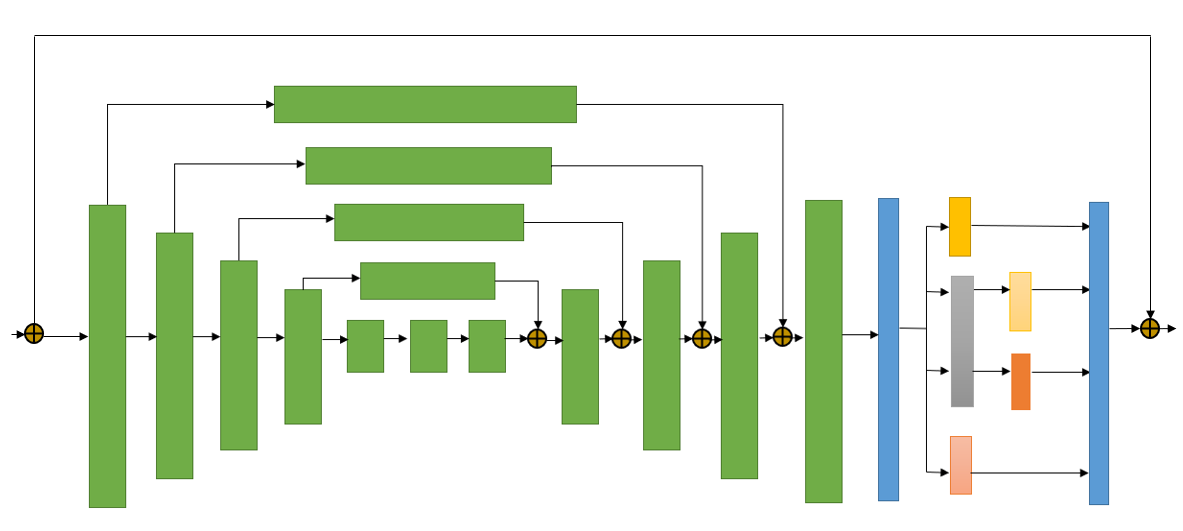
\includegraphics[width = 0.6\textwidth, height=0.2\textheight]{images/hourglass1.PNG}} &
{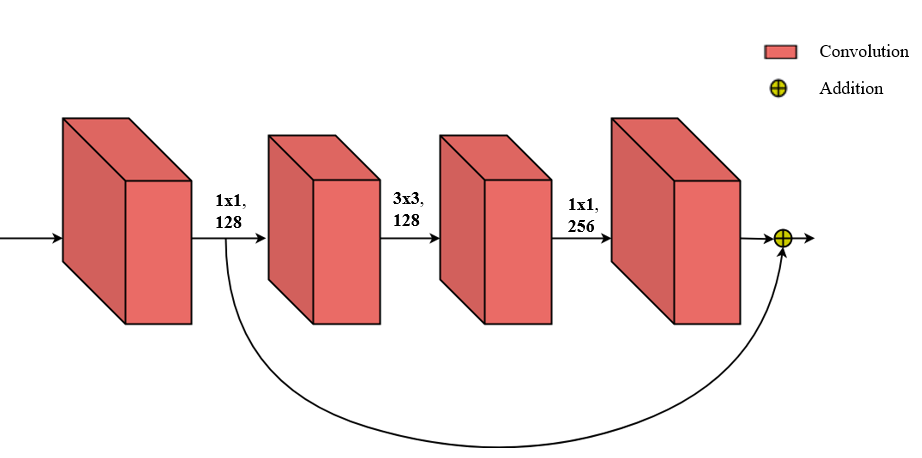
\includegraphics [width = 0.4\textwidth, height= 0.15\textheight]{images/Residualunit.PNG}} \\
(a) & (b) \\
% \caption{Residual-unit used throughout the stacked hourglass architecture. The first layer has 256 feature maps which are mapped down to 128 using a bottle-neck layer. After convolution using a $3 \times 3$ filter, these features maps are mapped back to 256 and added to the input feature maps to produce the final feature maps of this unit.}
% \label{fig:my_labelx}
\end{tabular}
\end{figure*}

\begin{figure*}[ht]
\begin{tabular}{c}
{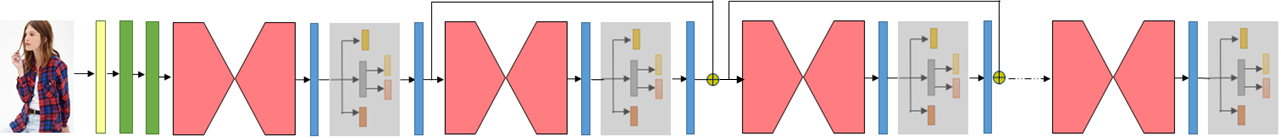
\includegraphics[width = 1\textwidth, height=0.1\textheight]{images/stack.png}} \\
{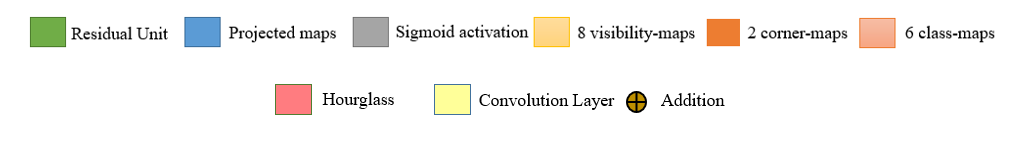
\includegraphics[width = 1\textwidth, height=0.1\textheight]{images/legends.PNG}} \\
(c)
\label{fig:my_label71}
\end{tabular}
\caption{Stacked hourglass architecture. (a) Stacked hourglass module consisting of residual units with bottom up and top-down processing; (b) architecture of residual unit with skip connections (c) Overall cascaded stacked hourglass architecture pipeline with intermediate supervision. }
\end{figure*}


\section{Experiments}
 DeepFashion dataset has about 123,000 images, richly annotated to support multiple tasks like landmark detection, apparel classification and apparel detection for fashion analysis.
%  Table~\ref{table:table2} represents the data-distribution of the dataset. 
 These annotations contain eight landmarks; three high-level apparel categories, i.e., upper (e.g., shirts), lower (e.g., pants) and full-body (e.g., dresses) apparels depending upon the body-parts they are designed for; five viewpoint variations, i.e., normal, medium or large and medium zoom-in or large zoom-in poses.
Also, since the landmarks on the apparels are frequently occluded in images, these annotations also contain the visibility status of the landmarks, indicating the occluded, visible, truncated and non-existent landmarks respectively. Truncated landmarks mean that the landmark exists in the apparel but has been cropped in the image and non-existent landmark means that the landmark does not exist for this particular apparel, e.g., the left and right collar or the left and right sleeve do not exist in a lower-body apparel like pants. 
% Table~\ref{table:table1} represents the existing and non-existing landmarks in each category. 
But for the training purposes, we consider all the visibility states other than visible as occluded, hence  $\gamma \in \{0,1\}$, where values 1 and 0 indicate the visible and the occluded landmarks respectively. 
 
% \begin{table}[ht]
% \centering
% \caption{Data Distribution in DeepFashion.}
% \footnotesize
% \begin{tabular}{|p{2cm}|p{2cm}|p{2cm}|p{2cm}|p{2cm}|}
% \hline
% \textbf{Category} & \textbf{Total} & \textbf{Train} & \textbf{Validation} & \textbf{Test}\\[2pt]
% \hline
% \textbf{upper} &   42031  & 28283   & 6873 & 6875\\[1pt]
% \hline
% \textbf{lower}  & 30972 & 20925 & 5027 & 5020\\[1pt]
% \hline
% \textbf{full}  & 50013 & 33825 & 8092 & 8096\\[1pt]
% \hline
% \textbf{overall}  &123016 &83033  & 19992  & 19991\\[1pt]
% \hline
% \end{tabular}
% \label{table:table2}
% \end{table}
We use Normalized Error and Percentage Landmark Detection metrics to evaluate and compare our results for landmark detection. 

\begin{enumerate}

\item \textbf{Normalized Error (NE) :} NE is the $l_2$ distance  $\norm{a^{i}_{p} - \hat{a^{i}_{p}}}^2$ between the predicted and the ground truth landmarks in the normalized coordinate space (i.e. divided by height/width of the image). Smaller values of NE mean better results.
% \begin{align}
% NE^N_{P} \big( a , \hat{a} \big)  = \frac{1}{N} \frac{1}{P} \sum_{i = 1}^{N} \sum_{p = 1}^{P} \frac{\norm{a^{i}_{p} - \hat{a^{i}_{p}}}^2}{m}
% \end{align}
\item \textbf{Percentage Landmark Detection (PLD):} is calculated as percentage of detected visible  landmarks with normalized error under the threshold $\eta$. In our experiments, we take $\eta = 0.5$. However, Figure \ref{fig:my_labeln} shows the NE vs PLD graph on different values of $\eta$ on the stacked hourglass network. This shows that the accuracy increases with more tolerant thresholds like 0.7.   
 
% % \begin{center}
% \begin{equation}
% \scriptsize
% \begin{split}
% PLD^N_{P} \big( a , \hat{a} \big) =  \frac{\countB \Bigg( \;\frac{\norm{a^i_p - \hat{a^{i}_p}}^2}{m} < \eta \;\Bigg)}{N * P} \times 100,
% \\
% i \in \{1, \dots, N\},\;\; p \in \{1, \dots, P\}.   
% \end{split}
% \end{equation} 
% % \end{center}
 
\end{enumerate}

For the landmarks' visibility, we calculate the percentage of visibility (PLDv) states classified correctly. The apparel's bounding box localization and the apparel classification tasks are jointly evaluated using average precision (AP) metrics, popularly used in COCO \cite{lin2014microsoft} and PASCAL VOC object \cite{everingham2010pascal}  detection tasks. AP is the measure of intersection over union (IOU) of the predicted and the ground truth bounding box calculated using Jaccard distance \cite{sulaiman2012jaccard}.

\textbf{Experimental Settings:} The input images are re-sized to $256 \times 256$ resolution, and two initial residual units with $7 \times 7$ kernels bring the resolution down to $64 \times 64$. In the hourglasses, residual units use only $3 \times 3$ kernels. After the top-down processing each stacked hourglass reaches down to the feature maps of  resolution $4 \times 4$. All the architectures are implemented using Torch and optimized with Adam optimizer. The learning rate starts at 0.0007 and decreases by 10 after the validation accuracy pleatues. We train each architecture for 100 epochs with batch size 10. The values of $\nu_1, \nu_2, \nu_3, \nu_4$ in equation (6) are set to 1 to provide equal weightage to the losses.
We  use only 2 hourglasses for training because as demonstrated in \cite{xiao2018simple}, using more that 2 hourglasses causes saturation. Testing is performed with PLD thresholds $\eta = 0.5$. 
In order to avoid over-fitting, we also perform data augmentation on the training set while training as a Markov process, i.e., the augmentation is performed via a sequence of random transformations such as scaling, rotation, flipping, and adding color noise, on the images from the training set, with parameters drawn randomly from hand-tuned ranges. We empirically choose the interval $[-45,45]$ degrees for rotation, $[0.75,1.25]$ for scaling.   

 Table~\ref{table:table1} and Table~\ref{table:table10}  represents the NE scores and PLD scores respectively for the landmarks in DeepFashion test set using stacked hourglass network (SHG). Table~\ref{table:table1} compares normalized error of the stacked hourglass network with the Deep Fashion Alignment (DFA) network proposed in \cite{liu2016fashion}. Only NE scores are provided by DFA on this dataset. Stacked hourglass network demonstrates a significant improvement over DFA. Since previous works are not open source and lack implementation details, we are not able to replicate them to benchmark PLD scores. We also try two different variations of stacked hourglass network, i.e., stacked hourglass network created using pyramid residual modules (SHGp) \cite{yang2017learning} and  stacked hourglass network created using cascade pyramid fusion (SHGc) \cite{he2015spatial}. We observe that stacked hourglass network using pyramid residual modules performs slightly better than the traditional stacked hourglass, but it introduces a lot many parameters to learn, hence it takes more time to train.
 
 \begin{table}[ht]
    \centering
     \scriptsize
    \caption{NE comparison on DeepFashion test set}
    \begin{tabular}{|p{0.9cm}|p{0.55cm}|p{0.6cm}|p{0.55cm}|p{0.6cm}|p{0.5cm}|p{0.5cm}|p{0.5cm}|}
    \hline
    \textbf{Method} & \textbf{l.collar} & \textbf{r.collar} & \textbf{l.sleeve} &  \textbf{r.sleeve} & \textbf{l.hem} & \textbf{r.hem} & \textbf{Avg} \\[5pt]
    \hline
    DFA \cite{liu2016fashion} & 0.048 & 0.048 & 0.091 & 0.089  & 0.071  & 0.072 & 0.068 \\[4pt]
    \hline
    SHG   & 0.023 & 0.025 & 0.042 & 0.046  & 0.032 & 0.036 & 0.034 \\[4pt]
    \hline
    \end{tabular}
    \label{table:table1}
\end{table}
 
\begin{table}[ht]
    \centering
    \tiny
    \caption{PLD comparison on DeepFashion test set at $\eta = 0.5$.}
    \begin{tabular}{|p{0.5cm}|p{0.5cm}|p{0.5cm}|p{0.5cm}|p{0.5cm}|p{0.4cm}|p{0.4cm}|p{0.4cm}|p{0.4cm}|p{0.3cm}|}
    \hline
    \textbf{Method} & \textbf{l.collar} & \textbf{r.collar} & \textbf{l.sleeve} &  \textbf{r.sleeve} &\textbf{l.waist} &\textbf{r.waist} &\textbf{l.hem}& \textbf{r.hem} & \textbf{$\sum$} \\ [5pt]
    \hline
     SHG  & 86.9 & 87.1& 77.2 & 77.8  & 78.4 & 78.2 & 85.1  & 84.1  & 81.8 \\[4pt]
    \hline
    SHGp  & 87.3 & 87.3 & 77.5 & 78.1 & 78.7 & 78.6 & 85.3 & 84.4 & 82.1 \\[4pt]
    \hline
     SHGc  &  86.2  &	86.6  &	76.2  &	77.5  &	77  &	76.9	 & 84.1  &	83.1  &	81\\[4pt]
     \hline
     \end{tabular}
     \label{table:table10}
 \end{table}
 Also, among all the landmarks in the fashion items, the left and the right collar are the most easy to localize, whereas, the left and right sleeve and the left and right waist are the most difficult to localize. This might be because of the variability in the designs of the upper-body apparels.   e.g., T-shirt, tank-tops, camisoles, shirts, etc. have a huge variation in the location of the landmarks.  

\begin{figure}[ht]
\centering
{\includesvg [width = 0.5\textwidth, height= 0.2\textheight]{images/NE.svg}} \\
\caption{Normalized Error (NE) vs Percentage Landmark Detection (PLD) for stacked hourglass network }
\label{fig:my_labeln}
\end{figure}

Table~\ref{table:table14} lists  PLDv scores for all the landmarks on DeepFashion test set. 
Figure~\ref{fig:label12} represents the ground truth and predicted analysis on many images from the test set. On qualitative analysis, we observed that when the landmarks are in the image but are occluded as shown in Figure~\ref{fig:label12} (d, e, f), the network is able to learn subtle patterns in occlusion and set the visibility flag accordingly. E.g., while predicting the right and left collars, most of the occlusion in the front facing and the side facing images come from the hair, and there is often a small offset between the collar locations covered by the hair and the collar locations not covered by the hair.  Images in Figure~\ref{fig:label12} (d, g) compare the ground truth and predicted landmarks on some upper-body apparels and as it turns out, the visibility state is often predicted correctly with respect to the predicted location of landmarks. We observed similar patterns in the predictions of the landmarks where occlusion can be caused by some body parts. E.g., images in Figure~\ref{fig:label12} (f, i) have ground truth occlusion on the landmarks on the waist because of the back, arms and hands, but when the landmark locations are predicted with an offset, at a place that doesn't have such occlusion, the visibility state of the landmarks is predicted accurately. These would amount to some loss of quantitative accuracy in the visibility states of the landmarks, while these predictions are qualitatively sound. In addition to that, at some places, the faulty ground truth locations of the landmarks were also corrected. E.g., images in Figure~\ref{fig:label12} (j, k, l) have more accurate predicted landmarks than the ground truth landmarks.

\begin{table}[ht]
    \centering
     \tiny
    \caption{PLDv comparison on DeepFashion test set.}
    \begin{tabular}{|p{0.5cm}|p{0.5cm}|p{0.5cm}|p{0.5cm}|p{0.5cm}|p{0.4cm}|p{0.4cm}|p{0.4cm}|p{0.4cm}|p{0.3cm}|}
    \hline
    \textbf{Method} & \textbf{l.collar} & \textbf{r.collar} & \textbf{l.sleeve} & \textbf{r.sleeve} &\textbf{l.waist} &\textbf{r.waist} &\textbf{l.hem}& \textbf{r.hem} & \textbf{$\sum$} \\[4pt]
    \hline
    SHG  & 81.5 & 80.1 & 81.9 & 80.7 & 70.6 & 69.8 & 85.9 & 86.0  & 79.6 \\[3pt]
    \hline
    SHGp  & 81.7 & 80.3 & 82.2 & 80.8 & 70.8 & 70.2 & 85.9 & 86.2  & 79.4 \\[3pt]
    \hline
    SHGc& 80.4&	78.9&	80.8 &	79.4 &	69.6 &	69.6 &	84.8 &	85.0 &	78.5\\[3pt]
    \hline
    \end{tabular}
    \label{table:table14}
\end{table}

On the other hand, some error in the predictions come from the presence of upper-body apparels and the lower-body apparels in the same image. As shown in Figure~\ref{fig:label12} (m, p), the image contains landmarks of the upper-body apparel, but the network treats it like a full-body apparel and contains correct landmark predictions for the hems as well. Similarly, Figure~\ref{fig:label12} (n, q) has a lower-body apparel classified as full and upper-body apparel. While calculating the accuracy of the predicted landmark locations, we only consider the visible landmarks, so this does not impact the PLD accuracy for the landmarks, but it does impact the accuracy of the visibility states of all the landmarks. This also shows the scalability of this network to a dataset that contains the annotations of the landmarks of all the apparels in the images.
\begin{table}[ht]
    \centering
     \scriptsize
    \caption{The AP score for apparel detection on DeepFashion test set.}
    \begin{tabular}{|c|c|c|c|c|}
    \hline
    \textbf{Method} & \textbf{upper} & \textbf{lower} & \textbf{full}  & \textbf{AP} \\[3pt]
    \hline
    SHG   & 59.8 & 61.2  & 52.7 & 57.9 \\[2pt]
    \hline
    % SHGp   & 61.0 & 63.2  & 53.2 & 58.9  \\[5pt]
    %  \hline
    % SHGc  & 58.4 & 60.4  & 51.9 & 56.1  \\[5pt]
    % \hline
    SSD  & 53.2 & 55.7  & 50.8 & 53.0  \\[2pt]
    \hline
    R-CNN  & 53.2 & 55.7  & 50.9 & 53.2 \\[2pt]
    \hline
    \end{tabular}
    \label{table:table15}
\end{table}

\begin{figure*}
\centering
\begin{tabular} {cccccc}
% \hline
{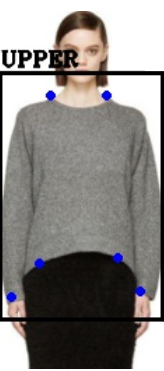
\includegraphics[align=c, width = 0.5in, height= 3cm]{images/gt_1.png}} & 
{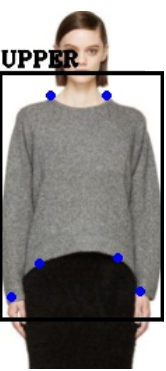
\includegraphics[align=c, width = 0.5in, height= 3cm]{images/p_1.png}} &
{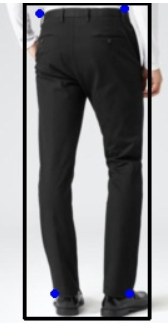
\includegraphics[align=c, width = 0.6in, height= 3cm]{images/gt_2.PNG}} &
{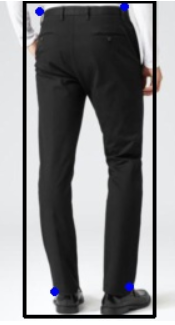
\includegraphics[align=c, width = 0.6in, height= 3cm]{images/p_2.PNG}} &
{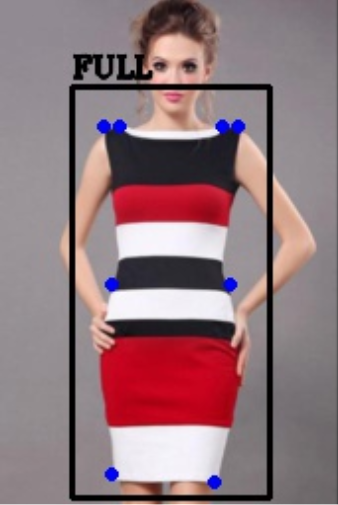
\includegraphics[align=c, width = 0.8in, height= 3cm]{images/gt_3.PNG}} & 
{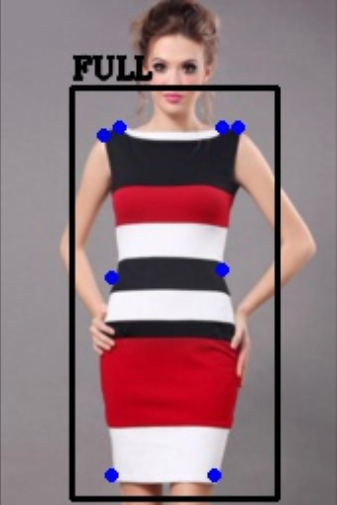
\includegraphics[align=c, width = 0.8in, height= 3cm]{images/p_3.PNG}}\\
% \hline 
(a) &  & (b) & & (c) &\\
% \hline
{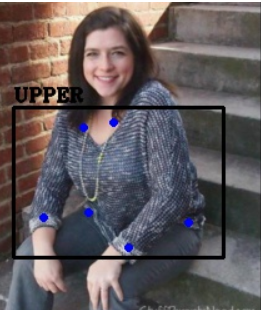
\includegraphics[align=c, width = 0.9in, height= 3cm]{images/gt_4.PNG}} &
{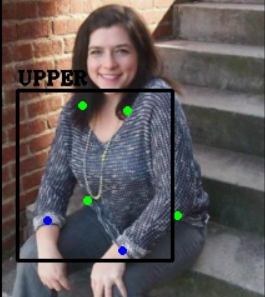
\includegraphics[align=c, width = 0.9in, height= 3cm]{images/p_4.PNG}} &
{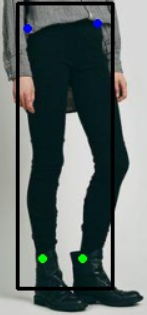
\includegraphics[align=c, width = 0.6in, height= 3cm]{images/gt_5.PNG}} &
{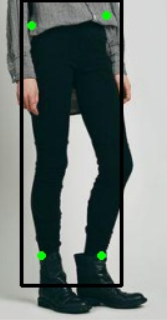
\includegraphics[align=c, width = 0.6in, height= 3cm]{images/p_5.PNG}} &
{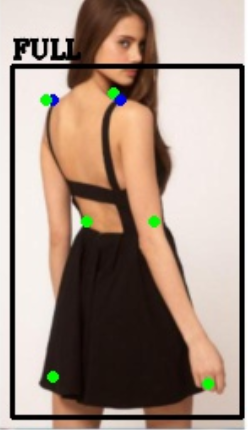
\includegraphics[align=c, width = 0.7in, height= 3cm]{images/gt_6.PNG}} &
{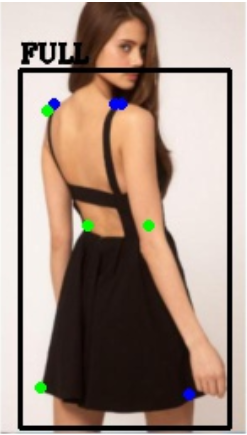
\includegraphics[align=c, width = 0.7in, height= 3cm]{images/p_6.PNG}} \\
% \hline 
(d) &  & (e) & & (f) &\\
% \hline
{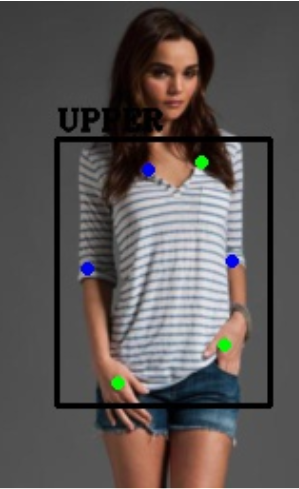
\includegraphics[align=c, width = 0.8in, height= 3cm]{images/gt_7.PNG}} &
{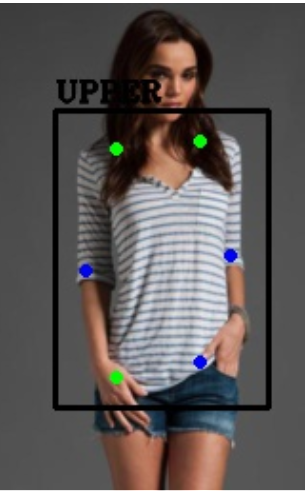
\includegraphics[align=c, width = 0.8in, height= 3cm]{images/p_7.PNG}} &
{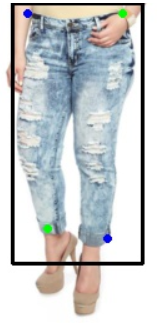
\includegraphics[align=c, width = 0.6in, height= 3cm]{images/gt_8.PNG}} &
{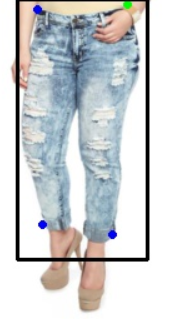
\includegraphics[align=c, width = 0.6in, height= 3cm]{images/p_8.PNG}} &
{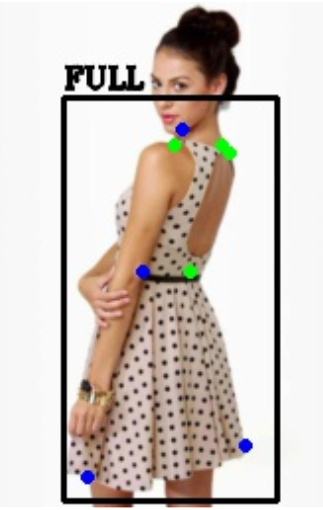
\includegraphics[align=c, width = 0.8in, height= 3cm]{images/gt_9.PNG}} &
{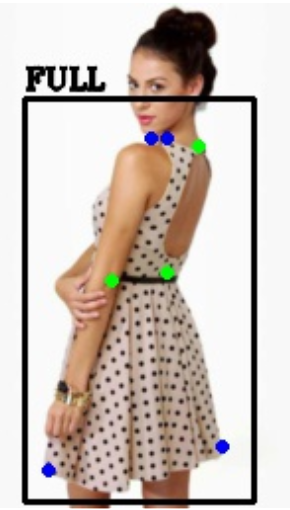
\includegraphics[align=c, width = 0.8in, height= 3cm]{images/p_9.PNG}} \\
% \hline 
(g) &  & (h) & & (i) &\\
% \hline
{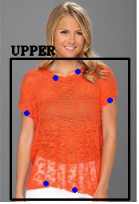
\includegraphics[align=c, width = 0.8in, height= 3cm]{images/gt_10.PNG}} &
{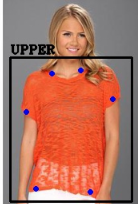
\includegraphics[align=c, width = 0.8in, height= 3cm]{images/p_10.PNG}} &
{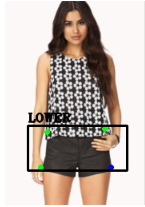
\includegraphics[align=c, width = 0.8in, height= 3cm]{images/gt_11.PNG}} &
{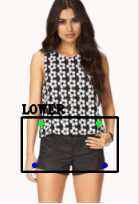
\includegraphics[align=c, width = 0.8in, height= 3cm]{images/p_11.PNG}} &
{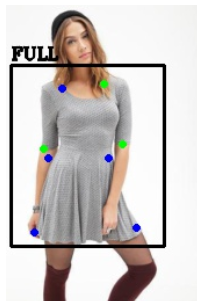
\includegraphics[align=c, width = 0.8in, height= 3cm]{images/gt_12.PNG}} &
{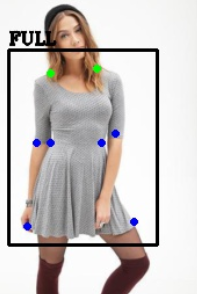
\includegraphics[align=c,  width = 0.8in, height= 3cm]{images/p_12.PNG}} \\
% \hline 
(j) &  & (k) & & (l) &\\
% \hline
{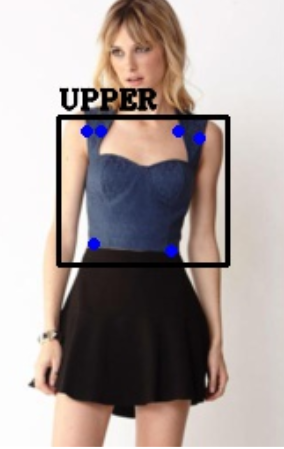
\includegraphics[align=c,  width = 0.75in, height= 3cm]{images/gt_13.PNG}} &
{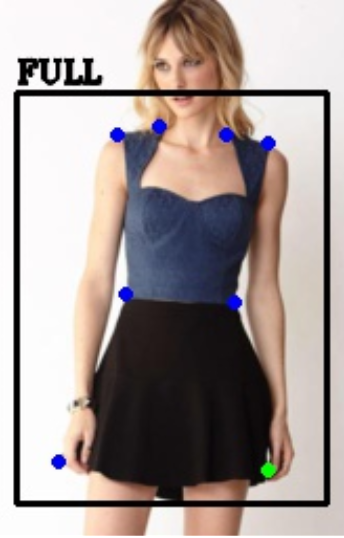
\includegraphics[align=c,  width = 0.8in, height= 3cm]{images/p_13.PNG}} &
{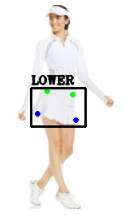
\includegraphics[align=c,  width = 0.8in, height= 3cm]{images/gt_14.PNG}} &
{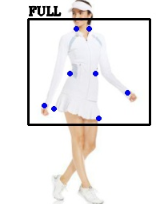
\includegraphics[align=c, width = 0.8in, height= 3cm]{images/p_14.PNG}} &
{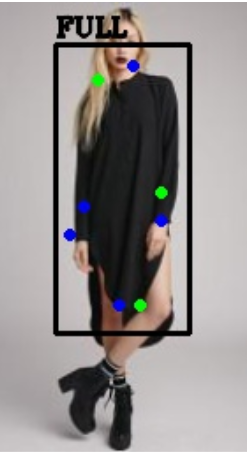
\includegraphics[align=c, width = 0.7in, height= 3cm]{images/gt_15.PNG}} &
{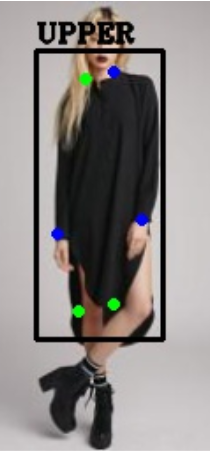
\includegraphics[align=c,  width = 0.7in, height= 3cm]{images/p_15.PNG}} \\
% \hline 
(m) &  & (n) & & (o) &\\
% \hline
{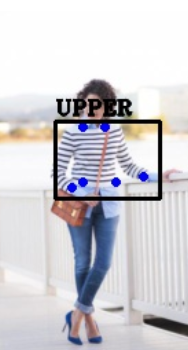
\includegraphics[align=c, width = 0.7in, height= 3cm]{images/gt_16.PNG}} &
{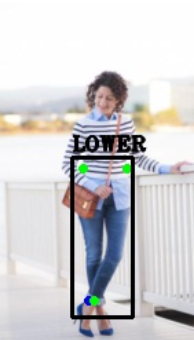
\includegraphics[align=c, width = 0.7in, height= 3cm]{images/p_16.PNG}} &
{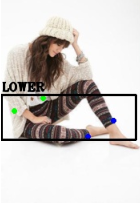
\includegraphics[align=c, width = 0.8in, height= 3cm]{images/gt_17.PNG}} &
{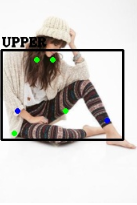
\includegraphics[align=c, width = 0.8in, height= 3cm]{images/p_17.PNG}} &
{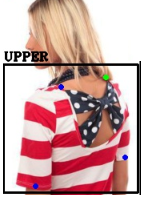
\includegraphics[align=c, width = 0.7in, height= 3cm]{images/gt_18.png}} &
{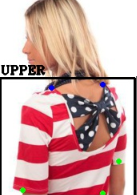
\includegraphics[align=c, width = 0.7in, height= 3cm]{images/p_18.png}} \\
% \hline 
(p) &  & (q) & & (r) &\\
% \hline
\end{tabular}
\caption{Sample images from DeepFashion test set. Left images in the image pair indicate the ground truth and the right images indicate the predicted apparel analysis. }
\label{fig:label12}
\end{figure*}

Table~\ref{table:table15} represents apparel detection AP score for all the landmarks. We also compare the results with standard SSD and R-CNN. We trained these architecture using transfer learning with the weight values obtained after training on COCO dataset \cite{lecun1999object}. Our proposed network trained from scratch does better than the other traditional object detection architectures. This is because of the rich features obtained via stacked hourglass architecture and more attention owing to to multi-task learning. We also compare the AP score of the multi-task learning with respect to different pose variations. As shown in Table~\ref{table:table16}, the AP scores are pretty good for normal, medium and large poses but the scores are very low for medium zoom-in and large zoom-in poses. 
\begin{table}[ht]
    \centering
    \scriptsize
    \caption{The AP score for apparel detection on different variations in the DeepFashion test set.}
    \begin{tabular}{|c|c|c|c|c|}
    \hline
    \textbf{Variation} & \textbf{upper} & \textbf{lower} & \textbf{full}  & \textbf{AP} \\[3pt]
    \hline
    Normal & 72.3 & 70.0 & 79.4 & 73.9   \\[2pt]
    \hline
    Medium & 80.5 & 75.1  & 73.7 & 76.4  \\[2pt]
    \hline
    Large  & 86.2 & 69.2 & 70.5 & 75.4 \\[2pt]
    \hline
    Medium zoom-in  & 33.7 & 27.7 & 20.0 &  27.1 \\[2pt]
    \hline
    Large zoom-in  & 55.3 & 63.6  & 53.3 & 57.4 \\[2pt]
    \hline
    \end{tabular}
    \label{table:table16}
\end{table}

Since  DeepFashion dataset contains annotation of only one apparel in an image, the images that contain both upper-body and lower-body apparels are subject to faulty detection as in Figure~\ref{fig:label12} (m, n, o, p, q) because the network has generalized over all the categories and would provide stronger detection for the more prominent apparel category in the image. However, the parameters behind decision of this prominence are unknown.  We also noticed that many upper-body apparels have been miss-classified as full-body apparels. This could be because these upper-body apparels, when paired with certain lower -body apparels, might look similar to full-body apparels as in Figure~\ref{fig:label12} (m). This, on one side indicates the ability of the network to learn generalized spatial features of the full-body apparels, but also indicates the difficulty to distinguish between the upper-body and full-body apparels. But in addition to these miss-classifications, we noticed that the predicted bounding boxes are more tightly bounded than the ground truth bounding boxes. Figure~\ref{fig:label12} (d, f, l, r) indicate some examples where the predicted bounding boxes more tightly localize the apparel than the ground-truth bounding boxes.

\section{Conclusion}
In this work, we demonstrated the use of a single architecture to perform the apparel detection as well as the apparel's landmark detection. We have shown that for fashion analysis, stacked hourglass architecture is comprehensive and it outperforms the state-of-the-art in both the tasks of  landmark detection and apparel detection. But this fashion analysis is limited by the dataset used in this work. There are some other datasets available for similar analysis like DeepFashion2 \cite{DeepFashion2}. The current dataset has only eight landmarks, where as DeepFashion2 dataset has 54 landmarks annotated for 13 different kind of apparels, along with the segmentation mask. Also, in DeepFashion, images only contain one apparel per image but this scenario is not very realistic. DeepFashion2 dataset has more than one apparel annotation per image. Stacked hourglass  architecture presented in this work can also be extended to predict the segmentation mask in parallel to the other tasks. Hence there is a lot of work that can be done in this domain, using this network on a more advanced dataset.

% \begin{figure}[ht]
% \centering
% \includegraphics[align=c,width = 8cm,height=6cm]{images/PLD_Accuracy_Upperbod.png}
%     \caption{Training PLDv score}
%     \label{fig:my_label}
% \end{figure}
%  \subsection{Apparel Detection}

% Hence, the medium-zoom in and the large zoom-in poses are the most difficult to detect and classify correctly.



\begin{thebibliography}{00}
\bibitem{huang2015cross} J. Huang, R. S. Feris, Q. Chen, and S. Yan, “Cross-domain image retrieval with
a dual attribute-aware ranking network,” in Proceedings of IEEE Conference on Computer Vision and Pattern Recognition, pp. 1062–1070, 2015.
\bibitem{he2016identity} K. He, X. Zhang, S. Ren, and J. Sun, “Identity mappings in deep residual networks,”
in European Conference on Computer Vision, pp. 630–645, Springer, 2016. 
\bibitem{liu2016deepfashion} S. Q. X. W. Ziwei Liu, Ping Luo and X. Tang, “Deepfashion: Powering robust
clothes recognition and retrieval with rich annotations,” in Proceedings of IEEE
Conference on Computer Vision and Pattern Recognition, June 2016.
\bibitem{liu2016fashion} Z. Liu, S. Yan, P. Luo, X. Wang, and X. Tang, “Fashion landmark detection in the
wild,” in European Conference on Computer Vision, pp. 229–245, Springer, 2016.
\bibitem{fu2012efficient}J. Fu, J.Wang, Z. Li, M. Xu, and H. Lu, “Efficient clothing retrieval with semanticpreserving
visual phrases,” in Asian Conference on Computer Vision, pp. 420–431,
Springer, 2012.
\bibitem{agarwal2018personalizing} P. Agarwal, S. Vempati, and S. Borar, “Personalizing similar product recommendations
in fashion e-commerce,” arXiv:1806.11371, 2018. 
\bibitem{wang2018attentive} W. Wang, Y. Xu, J. Shen, and S.-C. Zhu, “Attentive fashion grammar network for
fashion landmark detection and clothing category classification,” in Proceedings
of IEEE Conference on Computer Vision and Pattern Recognition, pp. 4271–4280,2018.
\bibitem{simo2016fashion} E. Simo-Serra and H. Ishikawa, “Fashion style in 128 floats: Joint ranking and
classification using weak data for feature extraction,” in Proceedings of IEEE Conference
on Computer Vision and Pattern Recognition, pp. 298–307, 2016.
\bibitem{gabale2018extract} V. Gabale and A. P. Subramanian, “How to extract fashion trends from social
media? a robust object detector with support for unsupervised learning,”
arXiv:1806.10787, 2018.
\bibitem{nakamura2018outfit} T. Nakamura and R. Goto, “Outfit generation and style extraction via bidirectional
lstm and autoencoder,” arXiv:1807.03133, 2018.
\bibitem{FashionTrends}  Aaron Orendorff, “Fashion industry-statistics, trends and strategy" https://www.shopify.com/enterprise/ecommerce-fashion-industry.
\bibitem{packer2018visually} C. Packer, J. McAuley, and A. Ramisa, “Visually-aware personalized recommendation
using interpretable image representations,” arXiv:1806.09820, 2018.
\bibitem{andriluka14cvpr} M. Andriluka, L. Pishchulin, P. Gehler, and B. Schiele, “2d human pose estimation:
New benchmark and state of the art analysis,” in Proceedings of IEEE Conference
on Computer Vision and Pattern Recognition, June 2014.
\bibitem{yan2017unconstrained}S. Yan, Z. Liu, P. Luo, S. Qiu, X. Wang, and X. Tang, “Unconstrained fashion landmark detection via hierarchical recurrent transformer networks,” in Proceedings of
the 25th ACM International Conference on multimedia, pp. 172–180, ACM, 2017.

\bibitem{talebi2018nima}H. Talebi and P. Milanfar, “Nima: Neural image assessment,” IEEE transactions
on image processing, vol. 27, no. 8, pp. 3998–4011, 2018.
\bibitem{newell2016stacked} A. Newell, K. Yang, and J. Deng, “Stacked hourglass networks for human pose
estimation,” in European Conference on Computer Vision, pp. 483–499, Springer,
2016.
\bibitem{lin2013network}M. Lin, Q. Chen, and S. Yan, “Network in network,”arXiv:1312.4400, 2013.
\bibitem{yang2017learning}W. Yang, S. Li, W. Ouyang, H. Li, and X. Wang, “Learning feature pyramids for human pose estimation,” in The IEEE International Conference on Computer Vision, vol. 2, 2017
\bibitem{lin2014microsoft}T.-Y. Lin, M. Maire, S. Belongie, J. Hays, P. Perona, D. Ramanan, P. Dollár, and C. L. Zitnick, “Microsoft coco: Common objects in context,” in European Conference on Computer Vision, pp. 740–755, Springer, 2014.
\bibitem{everingham2010pascal}M. Everingham, L. Van Gool, C. K. Williams, J. Winn, and A. Zisserman, “The pascal visual object classes (voc) challenge,” International Journal of Computer Vision, vol. 88, no. 2, pp. 303–338, 2010.
\bibitem{sulaiman2012jaccard}N. H. Sulaiman and D. Mohamad, “A jaccard-based similarity measure for soft sets,” in 2012 IEEE Symposium on Humanities, Science and Engineering Research, pp. 659–663, IEEE, 2012.
\bibitem{xiao2018simple}B. Xiao, H. Wu, and Y. Wei, “Simple baselines for human pose estimation and tracking,” in Proceedings of the european Conference on Computer Vision, pp. 466–481, 2018.
\bibitem{he2015spatial}K. He, X. Zhang, S. Ren, and J. Sun, “Spatial pyramid pooling in deep convolutional networks for visual recognition,” IEEE transactions on pattern analysis and machine intelligence, vol. 37, no. 9, pp. 1904–1916, 2015
\bibitem{chen2017adversarial}Y. Chen, C. Shen, X.-S. Wei, L. Liu, and J. Yang, “Adversarial posenet: A structure-aware convolutional network for human pose estimation,” in Proceedings of IEEE Conference on Computer Vision and Pattern Recognition, pp. 1212–1221, 2017.
\bibitem{andriluka20142d} M. Andriluka, L. Pishchulin, P. Gehler, and B. Schiele, “2d human pose estimation:
New benchmark and state of the art analysis,” in Proceedings of IEEE Conference
on Computer Vision and Pattern Recognition, pp. 3686–3693, 2014.
\bibitem{lecun1999object}Y. LeCun, P. Haffner, L. Bottou, and Y. Bengio, “Object recognition with gradientbased learning,” pp. 319–345, 1999.
\bibitem{zhang2019human} H. Zhang, H. Ouyang, S. Liu, X. Qi, X. Shen, R. Yang, and J. Jia, “Human pose
estimation with spatial contextual information,” arXiv:1901.01760, 2019.
\bibitem{jaderberg2015spatial} Zhang, Ziming, Rongmei Lin, and Alan Sullivan. "Deformable Part Networks." arXiv preprint arXiv:1805.08808 (2018).
\bibitem{chu2017multi}Chu, Xiao, et al. "Multi-context attention for human pose estimation." Proceedings of the IEEE Conference on Computer Vision and Pattern Recognition. 2017.
\bibitem{DeepFashion2}Y. Ge, R. Zhang, L. Wu, X. Wang, X. Tang, and P. Luo, “A versatile benchmark for detection, pose estimation, segmentation and re-identification of clothing images,”

\end{thebibliography}
\vspace{12pt}


\end{document}
